% put here just enough to compile it 
\documentclass{article}
\usepackage{xcolor}
\usepackage[english]{babel}
\usepackage{graphicx}
%\usepackage{docincludes}
\usepackage{siunitx}
\usepackage{hyperref}
\usepackage{cite}
\usepackage{amssymb}
\usepackage{amsmath}
\usepackage{amsmath}
\usepackage{tcolorbox}

\usepackage{todonotes} % use \todo{WP2Leader: xyz} \todo{ESRz: xyz} or \todo[inline]{} for simple notes.
%\usepackage{docincludes} %Added
\usepackage{mathtools} %Added for \prescript
\usepackage{algpseudocode}
\usepackage{algorithm}
\usepackage{enumitem}
\definecolor{deepblack}{rgb}{0,0,0}
\definecolor{deepblue}{rgb}{0,0,0.8}
\definecolor{deepred}{rgb}{0.6,0,0.4}
\definecolor{warningRed}{rgb}{1,0.2,0.2}
\definecolor{deepgreen}{rgb}{0,0.65,0}
\definecolor{commentgreen}{rgb}{0.5,0.7,0.5}

\usepackage{matlab-prettifier}




% is the format okay? format?? 
\usepackage[a4paper,top=2cm,bottom=2cm,left=3cm,right=3cm,marginparwidth=1.75cm]{geometry}
\title{Simulation of a simple crane lifting a load while rotating}

\begin{document}
\begin{titlepage}
\maketitle
\thispagestyle{empty}


\begin{center}

\includegraphics[scale=0.3]{Figures/thread-logo.pdf}
\end{center}

\begin{center}

\includegraphics[scale=0.3]{Figures/flag_yellow}
\end{center}
\vspace*{1.3cm}


\vspace*{1.3cm}
\begin{center}
\large{\sffamily{This project has received funding from the European Union's Horizon 2020 research and}}\\
\large{\sffamily{innovation programme under the Marie Sk{\l}odowska-Curie grant agreement No 860124.}}
\end{center}

\end{titlepage}
\tableofcontents
\newpage
%\input{methods.tex}
%\input{descriptionOfBeltDriveSimulation.tex}
%\input{descriptionOfCode_beltDrive.tex}

\section{Description of the simple crane model}

The example simulates the motion of a simple crane. The configuration of the system is shown in Figure~\ref{fig:ex_reeving_system}. The parameters of the system are given in Table~\ref{tab:reeving_system_parameters}. As sketched in Figure~\ref{fig:ex_reeving_system}, the system subjected to two imposed motions: rotation of the crane around the vertical $Z$ axis, or \textit{slewing motion}, and rotation of the drive reel to lift the payload, or \textit{winding motion}. The velocity profiles of the winding motion and slewing motion start at zero and smoothly reach a constant value following the laws: 

\begin{equation}
V = \left\{ {\begin{array}{*{20}{c}}
\frac{1}{2}V_c(1-\text{cos}(\frac{\pi t}{t_c}))&t < t_c\\
V_c&t \ge t_c
\end{array}} \right.
 \label{eq:rotation_angle}
\end{equation}


\begin{equation}
\Omega = \left\{ {\begin{array}{*{20}{c}}
\frac{1}{2}\Omega_c(1-\text{cos}(\frac{\pi t}{t_c}))&t < t_c\\
\Omega_c&t \ge t_c
\end{array}} \right.
 \label{eq:rotation_angle}
\end{equation}

\setlength{\parindent}{0cm}
where the assumed constant velocity values are $V_c = 1\, {\rm{m}}/{{\rm{s}}}$, and $\Omega_c = 0.3\, {\rm{rad}}/{{\rm{s}}}$, and the acceleration period is $t_c = 0.2 \,s$ for both motions.

\begin{table}[tbph]
    \caption{Reeving system parameters} \label{tab:reeving_system_parameters}
    \centering
    %\begin{tabular}{@{}lrlp{0.4\textwidth}@{}} \toprule
    \begin{tabular}{c|c|c|c} \hline
        Parameter & Value & Units & Description \\ \hline
        $d$ & 
            3 & \si{\meter} & 
            Distance between drive reel and deviation pulley \\
        $l_0$ & 
            8 & \si{\meter} & 
            Undeformed length of the vertical rope span at $t = 0$ \\
        $b$ & 
            0.3 & \si{\meter} & 
            Half side of cubic payload \\
        $R$ & 
            \num{0.1} & \si{\meter} & 
            Radius of the drive reel and deviation pulley \\
        $\rho A$ & 
            \num{0.6205} & \si{\kilo\gram\per\meter} & 
            Wire ropes linear density \\
        $EA$ & 
            \num{16.5} & \si{\mega\newton} & 
            Axial stiffness \\
        $EI$ & 
            \num{30.9} & \si{\newton\meter\squared} & 
            Bending stiffness \\
        $M$ & 
            1000 & \si{\kilo\gram} & 
            Mass of the payload \\ \hline
        %\bottomrule
    \end{tabular}
\end{table}

The simulation procedure is the Arbitrary Lagrangian-Eulerian Modal approach described in ~\cite{Escalona2022, Escalona2017}. All details about the formulation can be found in the reference papers. The model includes 1 rigid body which is the payload, and 2 wire-rope elements. The total set of coordinates is given by:

\begin{equation}
    {{\bf{p}}} = {\left[ {\begin{array}{*{20}{c}}{{\bf{q}}^{2}}^T & {{\bf{q}}^{a}}^T & {{\bf{q}}^{b}}^T \end{array}} \right]^T}
    \label{CoordinateS2}
\end{equation}

\setlength{\parindent}{0cm}
where ${{\bf{q}}^{2}}$ is the set of coordinates of rigid body 2. These are 3 transnational coordinates and 4 Euler parameters:

\begin{equation}
    {{\textbf{q}}}^{2} = {\left[ {\begin{array}{*{20}{c}}{\textbf{r}^{2}}^T&{\boldsymbol{\theta}^{2}}^T \end{array}} \right]^T}
\end{equation}

\begin{equation}
  {\textbf{r}}^{2} = {\left[ {\begin{array}{*{20}{c}}{{{{r}}_x^{2}}^T}&{{{{r}}_y^{2}}^T}&
  {{{{r}}_z^{2}}^T} \end{array}} \right]^T},     \boldsymbol{\theta}^{2} = {\left[ {\begin{array}{*{20}{c}}{{\theta_{0}^{2}}}&{{\theta_{1}^{2}}}&{{\theta_{2}^{2}}}&{{\theta_{3}^{2}}}\end{array}} \right]^T}  
\end{equation}

\begin{figure}
    \centering
    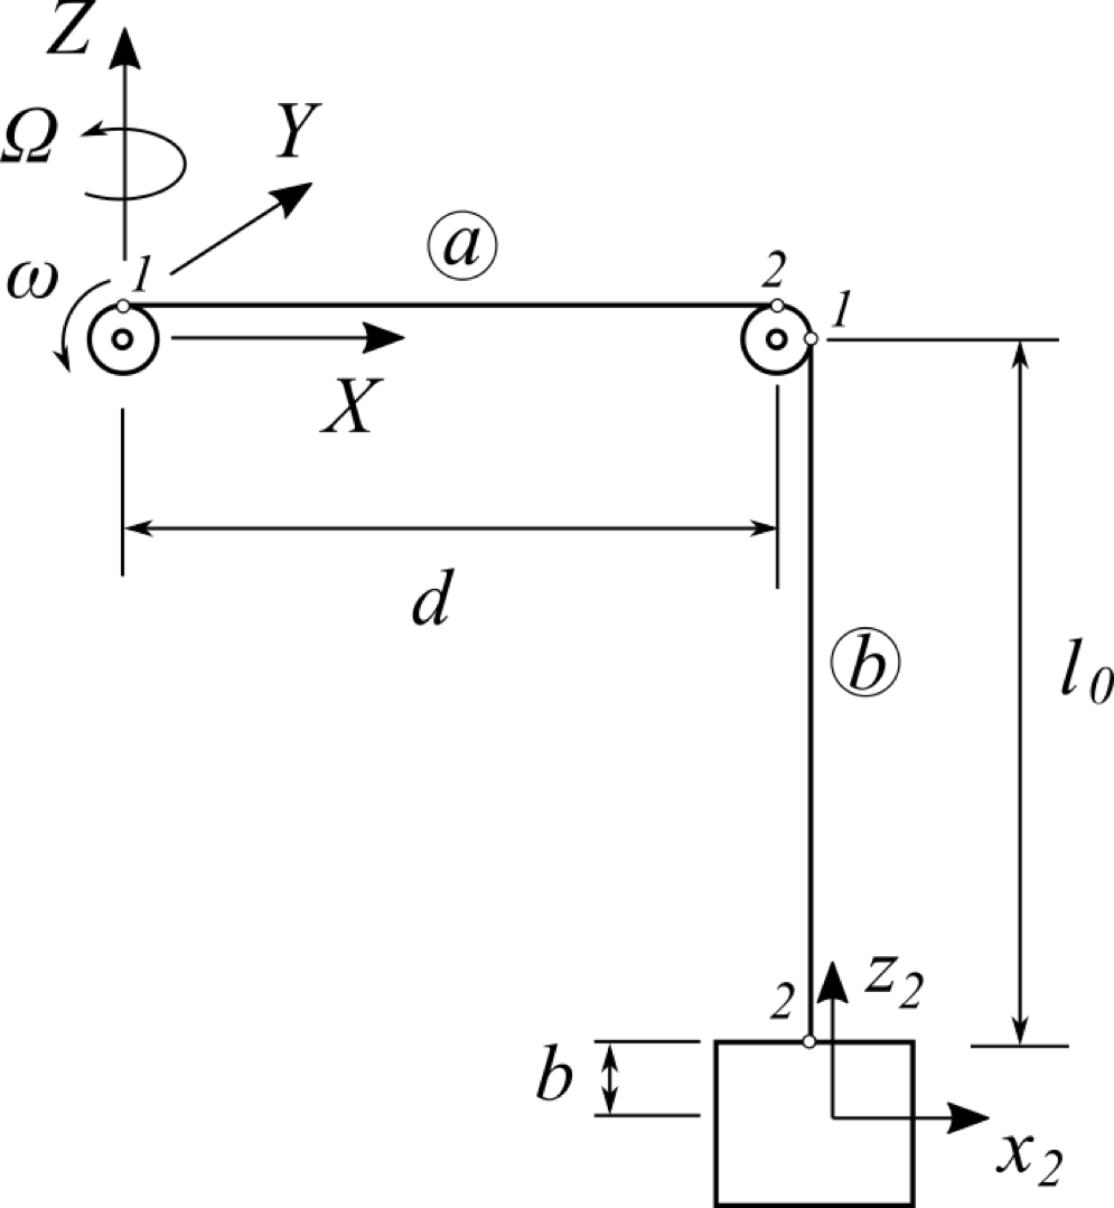
\includegraphics[width=0.4\textwidth]{Figures/simpleCrane.png}
    \caption{ALEM model of the reeving system of a simple crane}
    \label{fig:ex_reeving_system}
\end{figure}

Each ALEM wire-rope element $a$ and $b$ is kinematically described with a set of 6 absolute nodal coordinates $\textbf{q}_a$, 2 arc-length material coordinates $\textbf{q}_s$, and a maximum of 3 modal coordinates in each of the 3 local directions included in $\textbf{q}_m$. For example, for the wire-rope $a$, these coordinates are given by:

\begin{equation}
  {\textbf{q}}_a^{a} = {\left[ {\begin{array}{*{20}{c}}{{{\bf{q}}_a^{a}}^T}&{{{\bf{q}}_s^{a}}^T} & {{{\bf{q}}_m^{a}}^T} \end{array}} \right]^T}
\end{equation}

\begin{equation}
  {\textbf{q}}_a^{a} = {\left[ {\begin{array}{*{20}{c}}{{{\bf{r}}_1^{a}}^T}&{{{\bf{r}}_2^{a}}^T} \end{array}} \right]^T},     {\bf{q}}_s^{a} = {\left[ {\begin{array}{*{20}{c}}{{s_1^a}}&{{s_2^a}}\end{array}} \right]^T}  
\end{equation}

\begin{equation}
    {\textbf{q}}_m^{a} = \left[ {\begin{array}{*{20}{c}}{{q_{x,1}^a}}&{{q_{x,2}^a}} &{{q_{x,3}^a}}&{{q_{y,1}^a}}&{{q_{y,2}^a}}& {{q_{y,3}^a}}&{{q_{z,1}^a}}&{{q_{z,2}^a}}& {{q_{z,3}^a}}\end{array}} \right]^T 
\end{equation}

In this example, no modal coordinates are considered for the rope element $a$. For the rope element $b$, 3 axial-modal coordinates in the longitudinal direction $X_b$, $q_{mXi}^b,\, i = 1,2,3$, 1 transverse-modal coordinate in the local direction $Y_b$, $q_{mY1}^b$, and 1 transverse-modal coordinate in the local direction $Z_b$, $q_{mZ1}^b$, are used in the model. Therefore, the set of total coordinates $\textbf{p}$ is subjected to linear and nonlinear constraints. The linear constraints are expressed as:

\begin{equation} \label{Clin_Elev}
{{\bf{C}}_{lin}}\left( {{\bf{p}},t} \right) = \left[ {\begin{array}{*{20}{c}}
{{\bf{r}}_1^a - \left[ {\begin{array}{*{20}{c}}
0&0&R
\end{array}} \right]{}^T}\\
{{\bf{r}}_2^a - \left[ {\begin{array}{*{20}{c}}
{d\cos \alpha (t)}&{d\sin \alpha (t)}&R
\end{array}} \right]{}^T}\\
{{\bf{r}}_1^b - \left[ {\begin{array}{*{20}{c}}
{\left( {d + R} \right)\cos \alpha (t)}&{\left( {d + R} \right)\sin \alpha (t)}&0
\end{array}} \right]{}^T}\\
{{\bf{r}}_2^b - \left( {{{\bf{r}}^2} + {{\bf{A}}^2}\left[ {\begin{array}{*{20}{c}}
0&0&b
\end{array}} \right]{}^T} \right){}^T}\\
{s_1^a - \int {Vdt} }\\
{s_2^a - s_1^b}\\
{s_2^b - \left( {d + {l_0}} \right)}\\
{{\bf{q}}_m^a}\\
{q_{mY2}^b}\\
{q_{mY3}^b}\\
{q_{mZ2}^b}\\
{q_{mZ3}^b}
\end{array}} \right] = {\bf{0}}
\end{equation}

\setlength{\parindent}{0cm}
This is a set of 28 equations, $m_l = 28$.\\     

Nonlinear constraints are due to the force balance of the wire rope elements at the deviation sheave and to the unity of the quaternions used to describe the rotation of the payload, as follows: 

\begin{equation} 
{{\bf{C}}_{nonlin}}\left( {\bf{p}} \right) = \left[ {\begin{array}{*{20}{c}}
{F_{ax2}^a\left( {{{\bf{q}}^a}} \right) - F_{ax1}^b\left( {{{\bf{q}}^b}} \right)}\\
{{{\left( {\theta _0^2} \right)}^2} + {{\left( {\theta _1^2} \right)}^2} + {{\left( {\theta _2^2} \right)}^2} + {{\left( {\theta _3^2} \right)}^2} - 1}
\end{array}} \right] = {\bf{0}}
\label{WRnl}
\end{equation}

\setlength{\parindent}{0cm}
This is a set of 2 equations, $m_{nl} = 2$.\\

The number of generalized coordinates $\textbf{q}$ of the system , $n$, equals the number of coordinates in $\textbf{p}$, $n_p$, minus the number of linear constraints: $n = {n_p} - {m_l} = 41 - 28 = 13$.
The array $\textbf{q}$ is given by:

\begin{equation} \label{setq_Elev}
{\bf{q}} = {\left[ {\begin{array}{*{20}{c}}
{r_x^2}&{r_y^2}&{r_z^2}&{\theta _0^2}&{\theta _1^2}&{\theta _2^2}&{\theta _3^2}&{s_2^a}&{q_{mX1}^b}&{q_{mX2}^b}&{q_{mX3}^a}&{q_{mY1}^b}&{q_{mZ1}^b}
\end{array}} \right]^T}
\end{equation}

The generalized coordinates of the system $\textbf{q}$ is partitioned into independent coordinates, $\textbf{q}_{ind}$, and dependent coordinates, $\textbf{q}_{dep}$, as follows: 

\begin{equation} \label{subsetsq_Elev}
{{\bf{q}}^{ind}} = {\left[ {\begin{array}{*{20}{c}}
{r_x^2}&{r_y^2}&{r_z^2}&{\theta _0^2}&{\theta _1^2}&{\theta _2^2}&{q_{mX1}^b}&{q_{mX2}^b}&{q_{mX3}^a}&{q_{mY1}^b}&{q_{mZ1}^b}
\end{array}} \right]^T}
\end{equation}

\begin{equation} 
{{\mathbf{q}}^{dep}} = {\left[ {\begin{array}{*{20}{c}}
{{\theta_{0}^{3}}}&{s_2^a}
\end{array}} \right]^T}
\label{Dep}
\end{equation}

where the number of independent coordinates $n_{dep}$ equals the number of nonlinear constraints, $m_{nl}$. That way, the set $\textbf{q}_{dep}$ can be obtained solving the nonlinear constraints ${\bf{C}}_{nonlin}$ once the value of set $\textbf{q}_{ind}$ is known. Once the set $\textbf{q}$ is known, the linear constraints ${\bf{C}}_{lin}$ is used to find the value of the total set of coordinates $\textbf{p}$.








\section{Description of code}

The code implements a systematic formulation of the dynamics of wire-rope reeving systems modeled as flexible multibody systems using the arbitrary Lagrangian-Eulerian modal approach (ALEM) described in~\cite{Escalona2022}. This method can efficiently be used for the simulation of many industrial applications such as cranes, printers, elevators, and deployable structures for common operating conditions.

\subsection{Organization of the code}

The program is a set of Matlab files that has been grouped into 5 main sub-folders as:
\begin{itemize}
\item{\textbf{GeneralReevingSystems}: This folder contains the general m-files to simulate the dynamics of any reeving system.}
\item{\textbf{WireRopeForces}: This folder contains m-files that compute the forces and mass matrix of an ALEM  wire-rope element. These files have been generated using symbolic calculation in Matlab.}
\item{\textbf{Solver}: This folder contains a few numerical methods for equations solving that can be used as an alternative to the Matlab built-in functions.}
\item{\textbf{mexInterface}: This folder contains MEX files replace some m-files to decrease the computational time needed to solve the systems dynamics.}
\item{\textbf{simpleCrane}: This folder contains the m-files related to the presented example. These m-files describe the model parameters, coordinates, and the prescribed motion of the model. }
\end{itemize}

\subsection{Phases of simulation}

The phases of the simulation are described following the main file \textbf{simulateSimpleCrane.m} that can be found in the folder \textit{src/simpleCrane/}. The inputs and outputs of the used functions are described next. \\

\textbf{PHASE 1. Adding folders to Matlab path} \\

In the lines 1 - 5, the folders containing the m-files used in the simulation are added to the Matlab path, as follows:

\begin{tcolorbox}{{\begin{lstlisting}[style=Matlab-editor]
restoredefaultpath;
addpath("../../GeneralReevingSystems");
addpath("../../WireRopeForces");
addpath("../../mexInterface");
addpath("RB_kinematics");
\end{lstlisting}}
\end{tcolorbox} \\

\textbf{PHASE 2. Getting system parameters} \\

In line 8, the system parameters are stored in a data structure called \texttt{reevSys} that is the output of the function \textbf{CraneParams.m}. The different coordinate sets, the geometric, inertial and visco-elastic parameters of the system, the prescribed motion and the simulation parameters are defined and included as fields of the data structure \texttt{reevSys}. 

\begin{tcolorbox}{\begin{lstlisting}[style=Matlab-editor]
% Getting system parameters %
reevSys = CraneParams;
\end{lstlisting}}
\end{tcolorbox}\\

\setlength{\parindent}{0cm}
\textbf{Function:} \texttt{CraneParams.m} \\
\textbf{Input:} No input \\
\textbf{Output:} Data structure \texttt{reevSys} \\

\textbf{PHASE 3. Calculation of static equilibrium position} \\

The calculation of the static equilibrium position requires the solution of the non-linear algebraic equations in which the equations of motion turn when the generalized velocities and accelerations are set to zero. The unknowns of these equations are the value of the generalized coordinates and the Lagrange multipliers in static equilibrium. Lines 14 - 24 sets the initial guess of these variables. For the generalized coordinates, the initial guess is the reference value of the coordinates at the initial instant \texttt{qref}, corrected with an estimation of the rope deformation. For the Lagrange multipliers, a zero initial guess is used.

\begin{tcolorbox}{{\begin{lstlisting}[style=Matlab-editor]
% Reference value of coordinates (undeformed configuration) %
qref = [reevSys.d+reevSys.R 0.0 -(reevSys.l0 + reevSys.b) 1.0 0.0 0.0 0.0 reevSys.d 0.0 0.0 0.0 0.0 0.0]';
n = reevSys.n;

% Estimation of static displacement %
delta = reevSys.m2*9.81/(reevSys.EA/(reevSys.l0+reevSys.d));  % Elongation of both ropes
qref(3) = qref(3) - delta;  

% Initial guess of Lagrange multipliers associated with axial load
% constraint and Euler parameters %
lam = [0 0]';
\end{lstlisting}}
\end{tcolorbox}}

In lines 26 - 31, the static equilibrium position is calculated using the function \texttt{StaticEqReevingSystem.m}. Depending on the value of the parameter \texttt{reevSys.NLeq-method} different solvers can be used.

\begin{tcolorbox}{{\begin{lstlisting}[style=Matlab-editor]
% Calculation of static equilibrium position %
if strcmp(reevSys.NLeq_method,'NewtonRaphson')
    q0lam = NewtonRaphson(@StaticEqReevingSystem,[qref' lam']',reevSys);
elseif strcmp(reevSys.NLeq_method,'fsolve')
    q0lam = fsolve(@(qlam) StaticEqReevingSystem(qlam,reevSys),[qref' lam']',optimset('TolFun',1e-3));
end
\end{lstlisting}}
\end{tcolorbox}}

\setlength{\parindent}{0cm}
\textbf{Function:} \texttt{StaticEqReevingSystem.m} \\
\textbf{Inputs:} Array with generalized coordinates and Lagrange multipliers \texttt{qlam}. Data structure \texttt{reevSys.qdep0} \\
\textbf{Output:} Non-linear equilibrium equations \\

In lines 33 -41, the initial value of the independent generalized coordinates \texttt{qind0} and the initial guess of the dependent generalized coordinates \texttt{reevSys.qdep0} are extracted from the calculated static equilibrim position. Besides, the value of all coordinates at the static equilibrium position is obtained with function \texttt{CalculateAllCoordinates.m}.

\begin{tcolorbox}{{\begin{lstlisting}[style=Matlab-editor]
% Generalized coordinates in static equilibrium %
qst = q0lam(1:n,1);
% Initial value of independent coordinates %
qind0 = q0lam(reevSys.Ind);
% Initial guess of dependent coordinates %
reevSys.qdep0 = q0lam(reevSys.Dep);

% Calculation of all coordinates in static equilibrium %
pst = CalculateAllCoordinates(0.0,qst,reevSys);
\end{lstlisting}}
\end{tcolorbox}}

\setlength{\parindent}{0cm}
\textbf{Function:} \texttt{CalculateAllCoordinates.m} \\
\textbf{Inputs:} Time instant \texttt{t}. Generalized coordinates \texttt{q}. Data structure \texttt{reevSys.qdep0} \\
\textbf{Output:} Total set of coordinates \texttt{p} \\

Line 43 - 53 is a post-process of the static equilibrium position. The axial force field along the two rope elements is computed and plotted.

\begin{tcolorbox}{\begin{lstlisting}[style=Matlab-editor]
% Calculation of axial force field along rope %
sa = 0:0.01:qst(8);
for i = 1:length(sa)
    Pa(i) = AxialLoad(pst(7+1:7+17),sa(i),reevSys.EA_wr(1),reevSys);
end
sb = qst(8):0.01:(reevSys.d + reevSys.l0);
for i = 1:length(sb)
    Pb(i) = AxialLoad(pst(7+17+1:7+17+17),sb(i),reevSys.EA_wr(2),reevSys);
end

% Plots axial force field %
figure(10);
plot(sa,0.001*Pa,'b',sb,0.001*Pb,'g');
title('Axial load on wire ropes. Initial static position')
xlabel('Arc-length along rope (m)');
ylabel('Axial load (KN)');
legend('Horizontal element a','Vertical element b');
\end{lstlisting}}}
\end{tcolorbox}

\setlength{\parindent}{0cm}
\textbf{Function:} \texttt{AxialLoad.m} \\
\textbf{Inputs:} Nodal coordinates of the element \texttt{qi}. Arc-length coordinate \texttt{s}. Axial stiffness of the element \texttt{EA}. Data structure \texttt{reevSys.qdep0} \\
\textbf{Output:} Axial force \texttt{P} \\

\textbf{PHASE 4. Simulation} \\

Lines 65 - 78 perform the dynamic simulation. In line 66, the value of the independent velocities \texttt{vind} is set to zero. Depending on the value of the parameter \texttt{reevSys.ODE-method} different solvers for the equations of motion can be used.

\begin{tcolorbox}{\begin{lstlisting}[style=Matlab-editor]
% Initial value of independent velocities %
vind0 = zeros(size(reevSys.Ind));

if strcmp(reevSys.ODE_method,'ode15s')
    tspan = 0:0.001:5.0;
    options = odeset('MaxStep',0.001);
    [t y] = ode15s(@(t,y) EqMotReevingSystem(t,y,reevSys),tspan, [qind0' vind0']',options);
elseif strcmp(reevSys.ODE_method,'ode45')
     tspan = 0:0.001:5.0;
    options = odeset('MaxStep',0.001);
    [t y] = ode45(@(t,y) EqMotReevingSystem(t,y,reevSys),tspan, [qind0' vind0']',options);
elseif strcmp(reevSys.ODE_method,'RungeKutta4')
    [t y] = RungeKutta4(@EqMotReevingSystem,[0 5.0], [qind0' vind0']', 0.001, reevSys);
end
\end{lstlisting}}}
\end{tcolorbox}

\setlength{\parindent}{0cm}
\textbf{Function:} \texttt{EqMotReevingSystem.m} \\
\textbf{Inputs:} Time instant \texttt{t}. State vector \texttt{y} including independent coordinates \texttt{qind} and velocities \texttt{vind}. Data structure \texttt{reevSys} \\
\textbf{Output:} Independent accelerations \texttt{qind} \\

\textbf{PHASE 5. Post-process} \\

In lines 84 - 105, the total set of coordinates \texttt{p} at all instants and the axial loads at end $1$ of element $a$ and at end $2$ of element $b$ are computed and plotted. 

\begin{tcolorbox}{\begin{lstlisting}[style=Matlab-editor]
% Calculation of all coordinates all instants %
qdep = reevSys.qdep0;

p = zeros(reevSys.np,length(t));
% Axial load at end '1' of element 'a' %
P1 = zeros(length(t),1);
% Axial load at end '2' of element 'b' %
P2 = zeros(length(t),1);

for i = 1:length(t)
    [p(:,i), Cp, qdep] = Calculate_p_from_qind(t(i),y(i,1:length(reevSys.Ind))',qdep,reevSys);
    P1(i) = AxialLoad(p(7+1:7+17,i),p(7+16,i),reevSys.EA_wr(1),reevSys); 
    P2(i) = AxialLoad(p(7+17+1:7+17+17,i),p(7+17+17,i),reevSys.EA_wr(2),reevSys); 
end

% Plot time-history of axial loads %
figure(20);
plot(t,0.001*P1,'b',t,0.001*P2,'g')
title('Axial load on wire ropes')
xlabel('Time (s)');
ylabel('Axial load (KN)');
legend('End 1 of element a','End 2 of element b');
\end{lstlisting}}}
\end{tcolorbox}

\setlength{\parindent}{0cm}
\textbf{Function:} \texttt{Calculate-p-from-qind.m} \\
\textbf{Inputs:} Time instant \texttt{t}. State vector \texttt{y} including independent coordinates \texttt{qind} and velocities \texttt{vind}. Initial guess of dependent coordinates \texttt{qdep0}. Data structure \texttt{reevSys} \\
\textbf{Outputs:} Total set of coordinates \texttt{p}. Jacobian of nonlinear contraints \texttt{Cp}. Dependent coordinates \texttt{qdep} \\

In lines 107 - 121, the total set of coordinates are re-sampled (to avoid too long animation) and the animation of the motion of the crane is performed.

\begin{tcolorbox}{\begin{lstlisting}[style=Matlab-editor]
% Animation of crane motion %
% Number of frames of the animation %
N = 100;

% Resamples the data %
t2 = t(1):(t(end)-t(1))/(N-1):t(end);
p2 = zeros(reevSys.np,N);
for i = 1:reevSys.np
    p2(i,:) = interp1(t,p(i,:),t2);
end

% Animates the motion of the system %
for i = 1:length(t2)
    Fot(i) = AnimateCrane(t2(i),p2(:,i),reevSys);
end
\end{lstlisting}}}
\end{tcolorbox}

\setlength{\parindent}{0cm}
\textbf{Function:} \texttt{AnimateCrane.m} \\
\textbf{Inputs:} Time instant \texttt{t}. Total set of coordinates \texttt{p}. Data structure \texttt{reevSys} \\
\textbf{Outputs:} Video frame \texttt{Fot} \\


\section{Installation and running}
 This code does not require any installation. To execute it in a Matlab environment, simply run \textbf{simulateSimpleCrane.m} in \textit{src/simpleCrane/}. By running the code, the system solves the problem for the given parameters, plots simulation results and animates the motion of the crane. 


\begin{comment}
\subsection{m-files description}
\texttt{CalculateAllCoordinates}: The main structure of the code can be found in 

\textbf{Parameters} The set of the coordinates of the reeving system \texttt{p}, time vector \texttt{t}, and the parameters of the system as \texttt{reevSys}.

\textbf{Returns} The animation of the simulation
\end{comment}






\bibliographystyle{ieeetr}
%\typeout{}
\bibliography{literature}

\end{document}